\documentclass[../main.tex]{subfiles}


\begin{document}
\raggedright
Django is a Python based web framework which allows clean and pragmatic design as well as rapid development. The framework is designed to enable the coders to code without worrying about the security of the code as it guides the coders through securing the vulnerabilities such as SQL injection, cross-site scripting, cross-site request forgery and clickjacking. Django also has a user authentication system which can be customised to allow a secure way for data to be transferred\cite{django}. 

\subsection{Django vs Laravel}
Django is a Python based framework as stated above but Laravel\cite{laravel} on the other hand is a PHP based web framework. Django follows the Model View Template similar to Ruby on Rails but Laravel follows Object Oriented Programming as well as the Model View Template. In terms of website security, Django takes it extremely seriously and helps developers avoid the common mistakes which lead to the website having vulnerabilities while Laravel also has a guide to avoid making such mistakes but its contents are not as informative and detailed as Django. \\
Django is naturally very fast as it uses Python which is known for its speed and processing. Djano beats Laravels speed in all; Plaintext, JSON and SQLite Fetch\cite{djangovslaravel} as shown in \ref{fig:djangovslaravelsp}.

\begin{figure}[!htb]
        \center{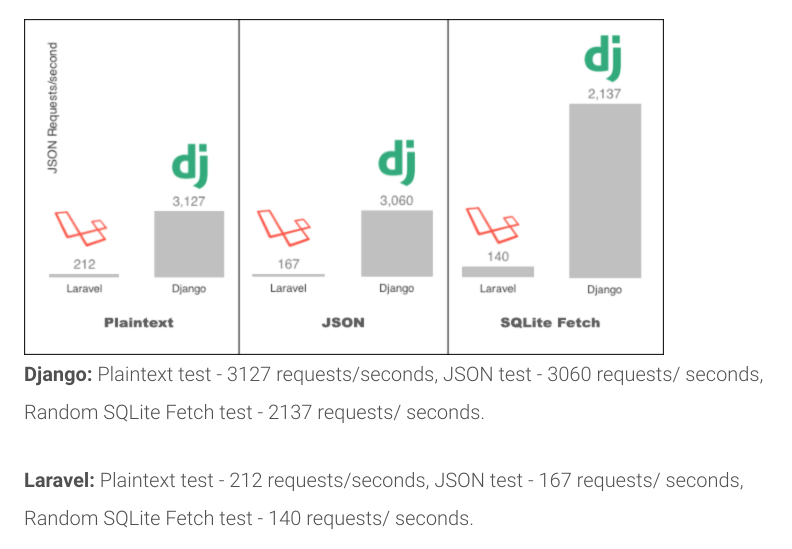
\includegraphics[scale=0.7]
        {images/djangovslaravelspeeds.png}}
        \caption{\label{fig:djangovslaravelsp} Django vs Laravel Speeds 2016 - CabotSolutions\cite{djangovslaravel}}
      \end{figure}
      
      
\subsection{Django vs Ruby on Rails} 
Both are popular web frameworks, Django more than Ruby on Rails for professional developers. They are open-source which allows all code to be customised in any way. Ruby on Rails allows the use of gems which are designed by other users, these come in handy when programming personal or individual projects however with professional projects licensing is a good idea to allow the code to be usable in the future\cite{djangovsrails}. 

Based on JetBrains research\cite{pythonresearch2018}\cite{rubyresearch2018} we know that Python is a really popular language compared to Ruby and it is highly used for Data Analysis and Web Development among various other things while developers use a mixture Ruby Versions which makes future updates to the code harder. Table \ref{tab:djangovsruby} shows the differences between Django and Ruby on Rails

\bgroup
\def\arraystretch{1.2}%  1 is the default, change whatever you need
\begin{table}[H]
\centering
\begin{tabular}{|l|l|l|}
\hline
& Django                                                                                                                                           & Ruby on Rails                                                                                                     \\ \hline
Pros       
& \begin{tabular}[l]{@{}l@{}}- Python is versatile \\ - Fast\\ - Caching System\\ - Data Analysis\\ - Great Security and \\ Autentication\end{tabular} 
& \begin{tabular}[l]{@{}l@{}}- Flexible\\ - Large Community\\ - Gems Available\\ - Easy Migration\end{tabular}      \\ \hline
Cons       
& \begin{tabular}[l]{@{}l@{}}- Hard to debug\\ - Monolithic architecture\end{tabular}                                                                   & \begin{tabular}[l]{@{}l@{}}- Bloated\\ - No Data Analysis\\ - Very explicit and \\ inelegant to read\end{tabular} \\ \hline
\end{tabular}
\captionof{table}{Django vs Ruby on Rails Pros and Cons \cite{djangovsrails}}\label{tab:djangovsruby} 
\end{table}
\egroup

\subsection{Summary}
Django, compared to various other web frameworks, is a good environment to use for the Extenuating Circumstance Forms because it provides security we are looking for, avoids vulnerabilities and is really fast when accessing and using with SQLite. Even with small or large numbers of data, it will be able to process it really quickly. Upgrading the system at a later stage will also be simple as Python is a highly developed language. 

\end{document}
